% Options for packages loaded elsewhere
% Options for packages loaded elsewhere
\PassOptionsToPackage{unicode}{hyperref}
\PassOptionsToPackage{hyphens}{url}
\PassOptionsToPackage{dvipsnames,svgnames,x11names}{xcolor}
%
\documentclass[
  letterpaper,
  DIV=11,
  numbers=noendperiod]{scrartcl}
\usepackage{xcolor}
\usepackage{amsmath,amssymb}
\setcounter{secnumdepth}{-\maxdimen} % remove section numbering
\usepackage{iftex}
\ifPDFTeX
  \usepackage[T1]{fontenc}
  \usepackage[utf8]{inputenc}
  \usepackage{textcomp} % provide euro and other symbols
\else % if luatex or xetex
  \usepackage{unicode-math} % this also loads fontspec
  \defaultfontfeatures{Scale=MatchLowercase}
  \defaultfontfeatures[\rmfamily]{Ligatures=TeX,Scale=1}
\fi
\usepackage{lmodern}
\ifPDFTeX\else
  % xetex/luatex font selection
\fi
% Use upquote if available, for straight quotes in verbatim environments
\IfFileExists{upquote.sty}{\usepackage{upquote}}{}
\IfFileExists{microtype.sty}{% use microtype if available
  \usepackage[]{microtype}
  \UseMicrotypeSet[protrusion]{basicmath} % disable protrusion for tt fonts
}{}
\makeatletter
\@ifundefined{KOMAClassName}{% if non-KOMA class
  \IfFileExists{parskip.sty}{%
    \usepackage{parskip}
  }{% else
    \setlength{\parindent}{0pt}
    \setlength{\parskip}{6pt plus 2pt minus 1pt}}
}{% if KOMA class
  \KOMAoptions{parskip=half}}
\makeatother
% Make \paragraph and \subparagraph free-standing
\makeatletter
\ifx\paragraph\undefined\else
  \let\oldparagraph\paragraph
  \renewcommand{\paragraph}{
    \@ifstar
      \xxxParagraphStar
      \xxxParagraphNoStar
  }
  \newcommand{\xxxParagraphStar}[1]{\oldparagraph*{#1}\mbox{}}
  \newcommand{\xxxParagraphNoStar}[1]{\oldparagraph{#1}\mbox{}}
\fi
\ifx\subparagraph\undefined\else
  \let\oldsubparagraph\subparagraph
  \renewcommand{\subparagraph}{
    \@ifstar
      \xxxSubParagraphStar
      \xxxSubParagraphNoStar
  }
  \newcommand{\xxxSubParagraphStar}[1]{\oldsubparagraph*{#1}\mbox{}}
  \newcommand{\xxxSubParagraphNoStar}[1]{\oldsubparagraph{#1}\mbox{}}
\fi
\makeatother

\usepackage{color}
\usepackage{fancyvrb}
\newcommand{\VerbBar}{|}
\newcommand{\VERB}{\Verb[commandchars=\\\{\}]}
\DefineVerbatimEnvironment{Highlighting}{Verbatim}{commandchars=\\\{\}}
% Add ',fontsize=\small' for more characters per line
\usepackage{framed}
\definecolor{shadecolor}{RGB}{241,243,245}
\newenvironment{Shaded}{\begin{snugshade}}{\end{snugshade}}
\newcommand{\AlertTok}[1]{\textcolor[rgb]{0.68,0.00,0.00}{#1}}
\newcommand{\AnnotationTok}[1]{\textcolor[rgb]{0.37,0.37,0.37}{#1}}
\newcommand{\AttributeTok}[1]{\textcolor[rgb]{0.40,0.45,0.13}{#1}}
\newcommand{\BaseNTok}[1]{\textcolor[rgb]{0.68,0.00,0.00}{#1}}
\newcommand{\BuiltInTok}[1]{\textcolor[rgb]{0.00,0.23,0.31}{#1}}
\newcommand{\CharTok}[1]{\textcolor[rgb]{0.13,0.47,0.30}{#1}}
\newcommand{\CommentTok}[1]{\textcolor[rgb]{0.37,0.37,0.37}{#1}}
\newcommand{\CommentVarTok}[1]{\textcolor[rgb]{0.37,0.37,0.37}{\textit{#1}}}
\newcommand{\ConstantTok}[1]{\textcolor[rgb]{0.56,0.35,0.01}{#1}}
\newcommand{\ControlFlowTok}[1]{\textcolor[rgb]{0.00,0.23,0.31}{\textbf{#1}}}
\newcommand{\DataTypeTok}[1]{\textcolor[rgb]{0.68,0.00,0.00}{#1}}
\newcommand{\DecValTok}[1]{\textcolor[rgb]{0.68,0.00,0.00}{#1}}
\newcommand{\DocumentationTok}[1]{\textcolor[rgb]{0.37,0.37,0.37}{\textit{#1}}}
\newcommand{\ErrorTok}[1]{\textcolor[rgb]{0.68,0.00,0.00}{#1}}
\newcommand{\ExtensionTok}[1]{\textcolor[rgb]{0.00,0.23,0.31}{#1}}
\newcommand{\FloatTok}[1]{\textcolor[rgb]{0.68,0.00,0.00}{#1}}
\newcommand{\FunctionTok}[1]{\textcolor[rgb]{0.28,0.35,0.67}{#1}}
\newcommand{\ImportTok}[1]{\textcolor[rgb]{0.00,0.46,0.62}{#1}}
\newcommand{\InformationTok}[1]{\textcolor[rgb]{0.37,0.37,0.37}{#1}}
\newcommand{\KeywordTok}[1]{\textcolor[rgb]{0.00,0.23,0.31}{\textbf{#1}}}
\newcommand{\NormalTok}[1]{\textcolor[rgb]{0.00,0.23,0.31}{#1}}
\newcommand{\OperatorTok}[1]{\textcolor[rgb]{0.37,0.37,0.37}{#1}}
\newcommand{\OtherTok}[1]{\textcolor[rgb]{0.00,0.23,0.31}{#1}}
\newcommand{\PreprocessorTok}[1]{\textcolor[rgb]{0.68,0.00,0.00}{#1}}
\newcommand{\RegionMarkerTok}[1]{\textcolor[rgb]{0.00,0.23,0.31}{#1}}
\newcommand{\SpecialCharTok}[1]{\textcolor[rgb]{0.37,0.37,0.37}{#1}}
\newcommand{\SpecialStringTok}[1]{\textcolor[rgb]{0.13,0.47,0.30}{#1}}
\newcommand{\StringTok}[1]{\textcolor[rgb]{0.13,0.47,0.30}{#1}}
\newcommand{\VariableTok}[1]{\textcolor[rgb]{0.07,0.07,0.07}{#1}}
\newcommand{\VerbatimStringTok}[1]{\textcolor[rgb]{0.13,0.47,0.30}{#1}}
\newcommand{\WarningTok}[1]{\textcolor[rgb]{0.37,0.37,0.37}{\textit{#1}}}

\usepackage{longtable,booktabs,array}
\usepackage{calc} % for calculating minipage widths
% Correct order of tables after \paragraph or \subparagraph
\usepackage{etoolbox}
\makeatletter
\patchcmd\longtable{\par}{\if@noskipsec\mbox{}\fi\par}{}{}
\makeatother
% Allow footnotes in longtable head/foot
\IfFileExists{footnotehyper.sty}{\usepackage{footnotehyper}}{\usepackage{footnote}}
\makesavenoteenv{longtable}
\usepackage{graphicx}
\makeatletter
\newsavebox\pandoc@box
\newcommand*\pandocbounded[1]{% scales image to fit in text height/width
  \sbox\pandoc@box{#1}%
  \Gscale@div\@tempa{\textheight}{\dimexpr\ht\pandoc@box+\dp\pandoc@box\relax}%
  \Gscale@div\@tempb{\linewidth}{\wd\pandoc@box}%
  \ifdim\@tempb\p@<\@tempa\p@\let\@tempa\@tempb\fi% select the smaller of both
  \ifdim\@tempa\p@<\p@\scalebox{\@tempa}{\usebox\pandoc@box}%
  \else\usebox{\pandoc@box}%
  \fi%
}
% Set default figure placement to htbp
\def\fps@figure{htbp}
\makeatother





\setlength{\emergencystretch}{3em} % prevent overfull lines

\providecommand{\tightlist}{%
  \setlength{\itemsep}{0pt}\setlength{\parskip}{0pt}}






\KOMAoption{captions}{tableheading}
\makeatletter
\@ifpackageloaded{caption}{}{\usepackage{caption}}
\AtBeginDocument{%
\ifdefined\contentsname
  \renewcommand*\contentsname{Table of contents}
\else
  \newcommand\contentsname{Table of contents}
\fi
\ifdefined\listfigurename
  \renewcommand*\listfigurename{List of Figures}
\else
  \newcommand\listfigurename{List of Figures}
\fi
\ifdefined\listtablename
  \renewcommand*\listtablename{List of Tables}
\else
  \newcommand\listtablename{List of Tables}
\fi
\ifdefined\figurename
  \renewcommand*\figurename{Figure}
\else
  \newcommand\figurename{Figure}
\fi
\ifdefined\tablename
  \renewcommand*\tablename{Table}
\else
  \newcommand\tablename{Table}
\fi
}
\@ifpackageloaded{float}{}{\usepackage{float}}
\floatstyle{ruled}
\@ifundefined{c@chapter}{\newfloat{codelisting}{h}{lop}}{\newfloat{codelisting}{h}{lop}[chapter]}
\floatname{codelisting}{Listing}
\newcommand*\listoflistings{\listof{codelisting}{List of Listings}}
\makeatother
\makeatletter
\makeatother
\makeatletter
\@ifpackageloaded{caption}{}{\usepackage{caption}}
\@ifpackageloaded{subcaption}{}{\usepackage{subcaption}}
\makeatother
\usepackage{bookmark}
\IfFileExists{xurl.sty}{\usepackage{xurl}}{} % add URL line breaks if available
\urlstyle{same}
\hypersetup{
  pdfauthor={Matthias König},
  colorlinks=true,
  linkcolor={blue},
  filecolor={Maroon},
  citecolor={Blue},
  urlcolor={Blue},
  pdfcreator={LaTeX via pandoc}}


\title{
\includegraphics[width=0.7\linewidth,height=\textheight,keepaspectratio]{images/libsbgnpy_large.png}}
\usepackage{etoolbox}
\makeatletter
\providecommand{\subtitle}[1]{% add subtitle to \maketitle
  \apptocmd{\@title}{\par {\large #1 \par}}{}{}
}
\makeatother
\subtitle{Python library for SBGN}
\author{Matthias König}
\date{2025-04-15}
\begin{document}
\maketitle


\subsection{SBGN}\label{sbgn}

\begin{itemize}
\tightlist
\item
  \textbf{Systems Biology Graphical Notation}
\item
  Standardise graphical notation used in maps of biological processes
\item
  \textbf{Process Description (PD)}: temporal courses of biochemical
  interactions in a network
\item
  \textbf{Entity Relationship (ER)}: all relationships between
  participates, regardless of the temporal aspects
\item
  \textbf{Activity Flow (AF)}: flow of information between biochemical
  entities in a network
\end{itemize}

\pandocbounded{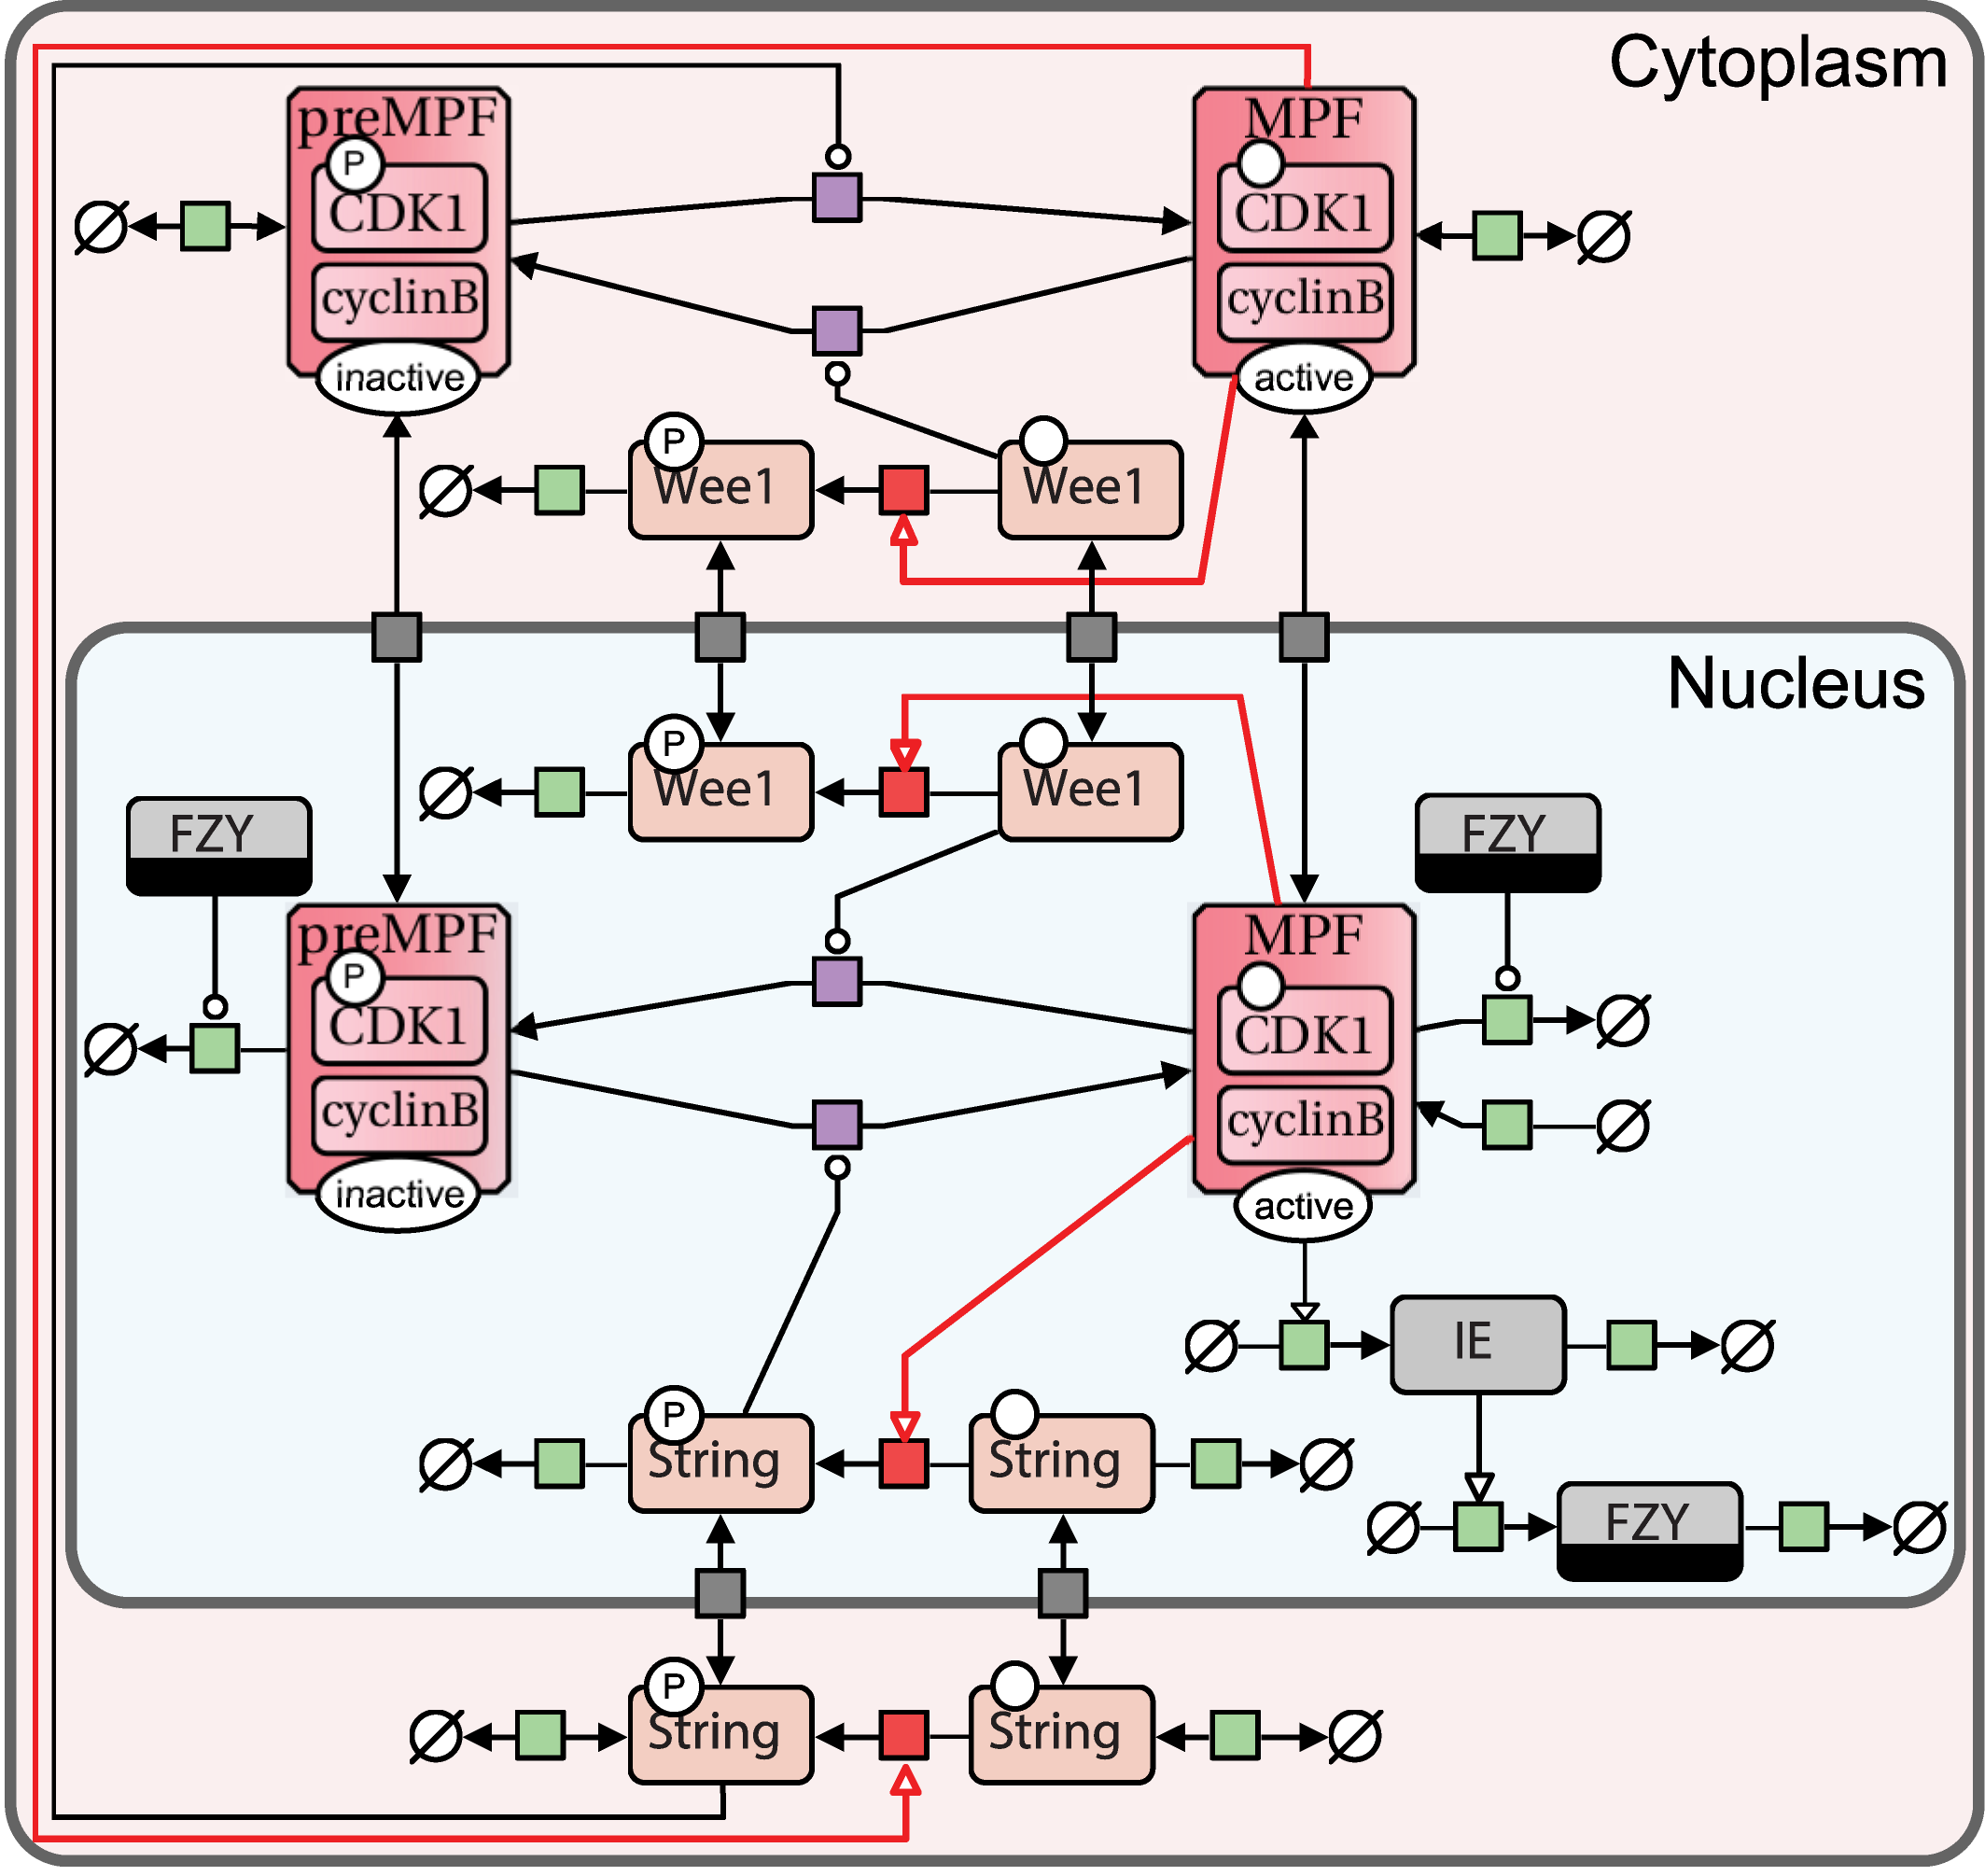
\includegraphics[keepaspectratio]{./images/toure_drosophila.png}}

\subsection{libsbgnpy}\label{libsbgnpy}

\begin{itemize}
\tightlist
\item
  Python library for SBGN
\item
  Supports AF, PD, ER
\item
  Supports libsbgn/0.3
\item
  \textbf{new}: support for render extension
\item
  \textbf{new}: python dataclasses with type annotations
\item
  \textbf{new}: py3.12, py3.13 support
\item
  \textbf{new}: more and better documentation:
  \url{https://matthiaskoenig.github.io/libsbgnpy/}
\end{itemize}

\pandocbounded{
\includegraphics[keepaspectratio]{./images/github_screenshot.png}}

\subsection{1. Create map}\label{create-map}

\begin{Shaded}
\begin{Highlighting}[]
\CommentTok{"""Glucokinase example."""}
\BuiltInTok{map} \OperatorTok{=}\NormalTok{ Map(}
\NormalTok{    language}\OperatorTok{=}\NormalTok{MapLanguage.PROCESS\_DESCRIPTION,}
\NormalTok{    bbox}\OperatorTok{=}\NormalTok{Bbox(x}\OperatorTok{=}\DecValTok{0}\NormalTok{, y}\OperatorTok{=}\DecValTok{0}\NormalTok{, w}\OperatorTok{=}\DecValTok{363}\NormalTok{, h}\OperatorTok{=}\DecValTok{253}\NormalTok{),}
\NormalTok{)}
\NormalTok{sbgn }\OperatorTok{=}\NormalTok{ Sbgn(}\BuiltInTok{map}\OperatorTok{=}\NormalTok{[}\BuiltInTok{map}\NormalTok{])}
\end{Highlighting}
\end{Shaded}

\subsection{2. Add glyphs}\label{add-glyphs}

\begin{Shaded}
\begin{Highlighting}[]
\CommentTok{"""Glucokinase example."""}
\BuiltInTok{map} \OperatorTok{=}\NormalTok{ Map(}
\NormalTok{    language}\OperatorTok{=}\NormalTok{MapLanguage.PROCESS\_DESCRIPTION,}
\NormalTok{    bbox}\OperatorTok{=}\NormalTok{Bbox(x}\OperatorTok{=}\DecValTok{0}\NormalTok{, y}\OperatorTok{=}\DecValTok{0}\NormalTok{, w}\OperatorTok{=}\DecValTok{363}\NormalTok{, h}\OperatorTok{=}\DecValTok{253}\NormalTok{),}
\NormalTok{)}
\NormalTok{sbgn }\OperatorTok{=}\NormalTok{ Sbgn(}\BuiltInTok{map}\OperatorTok{=}\NormalTok{[}\BuiltInTok{map}\NormalTok{])}

\CommentTok{\# Add glyphs}
\BuiltInTok{map}\NormalTok{.glyph.extend([}
\NormalTok{    Glyph(}
\NormalTok{        class\_value}\OperatorTok{=}\NormalTok{GlyphClass.SIMPLE\_CHEMICAL,}
        \BuiltInTok{id}\OperatorTok{=}\StringTok{"glyph1"}\NormalTok{,}
\NormalTok{        label}\OperatorTok{=}\NormalTok{Label(text}\OperatorTok{=}\StringTok{"Ethanol"}\NormalTok{),}
\NormalTok{        bbox}\OperatorTok{=}\NormalTok{Bbox(x}\OperatorTok{=}\DecValTok{40}\NormalTok{, y}\OperatorTok{=}\DecValTok{120}\NormalTok{, w}\OperatorTok{=}\DecValTok{60}\NormalTok{, h}\OperatorTok{=}\DecValTok{60}\NormalTok{),}
\NormalTok{    ),}
\NormalTok{    Glyph(}
\NormalTok{        class\_value}\OperatorTok{=}\NormalTok{GlyphClass.SIMPLE\_CHEMICAL,}
        \BuiltInTok{id}\OperatorTok{=}\StringTok{"glyph\_ethanal"}\NormalTok{,}
\NormalTok{        label}\OperatorTok{=}\NormalTok{Label(text}\OperatorTok{=}\StringTok{"Ethanal"}\NormalTok{),}
\NormalTok{        bbox}\OperatorTok{=}\NormalTok{Bbox(x}\OperatorTok{=}\DecValTok{220}\NormalTok{, y}\OperatorTok{=}\DecValTok{110}\NormalTok{, w}\OperatorTok{=}\DecValTok{60}\NormalTok{, h}\OperatorTok{=}\DecValTok{60}\NormalTok{),}
\NormalTok{    ),}
\NormalTok{    Glyph(}
\NormalTok{        class\_value}\OperatorTok{=}\NormalTok{GlyphClass.MACROMOLECULE,}
        \BuiltInTok{id}\OperatorTok{=}\StringTok{"glyph\_adh1"}\NormalTok{,}
\NormalTok{        label}\OperatorTok{=}\NormalTok{Label(text}\OperatorTok{=}\StringTok{"ADH1"}\NormalTok{),}
\NormalTok{        bbox}\OperatorTok{=}\NormalTok{Bbox(x}\OperatorTok{=}\DecValTok{106}\NormalTok{, y}\OperatorTok{=}\DecValTok{20}\NormalTok{, w}\OperatorTok{=}\DecValTok{108}\NormalTok{, h}\OperatorTok{=}\DecValTok{60}\NormalTok{),}
\NormalTok{    ),}
\NormalTok{    Glyph(}
\NormalTok{        class\_value}\OperatorTok{=}\NormalTok{GlyphClass.SIMPLE\_CHEMICAL,}
        \BuiltInTok{id}\OperatorTok{=}\StringTok{"glyph\_h"}\NormalTok{,}
\NormalTok{        label}\OperatorTok{=}\NormalTok{Label(text}\OperatorTok{=}\StringTok{"H+"}\NormalTok{),}
\NormalTok{        bbox}\OperatorTok{=}\NormalTok{Bbox(x}\OperatorTok{=}\DecValTok{220}\NormalTok{, y}\OperatorTok{=}\DecValTok{190}\NormalTok{, w}\OperatorTok{=}\DecValTok{60}\NormalTok{, h}\OperatorTok{=}\DecValTok{60}\NormalTok{),}
\NormalTok{    ),}
\NormalTok{    Glyph(}
\NormalTok{        class\_value}\OperatorTok{=}\NormalTok{GlyphClass.SIMPLE\_CHEMICAL,}
        \BuiltInTok{id}\OperatorTok{=}\StringTok{"glyph\_nad"}\NormalTok{,}
\NormalTok{        label}\OperatorTok{=}\NormalTok{Label(text}\OperatorTok{=}\StringTok{"NAD+"}\NormalTok{),}
\NormalTok{        bbox}\OperatorTok{=}\NormalTok{Bbox(x}\OperatorTok{=}\DecValTok{40}\NormalTok{, y}\OperatorTok{=}\DecValTok{190}\NormalTok{, w}\OperatorTok{=}\DecValTok{60}\NormalTok{, h}\OperatorTok{=}\DecValTok{60}\NormalTok{),}
\NormalTok{    ),}
\NormalTok{    Glyph(}
\NormalTok{        class\_value}\OperatorTok{=}\NormalTok{GlyphClass.SIMPLE\_CHEMICAL,}
        \BuiltInTok{id}\OperatorTok{=}\StringTok{"glyph\_nadh"}\NormalTok{,}
\NormalTok{        label}\OperatorTok{=}\NormalTok{Label(text}\OperatorTok{=}\StringTok{"NADH"}\NormalTok{),}
\NormalTok{        bbox}\OperatorTok{=}\NormalTok{Bbox(x}\OperatorTok{=}\DecValTok{300}\NormalTok{, y}\OperatorTok{=}\DecValTok{150}\NormalTok{, w}\OperatorTok{=}\DecValTok{60}\NormalTok{, h}\OperatorTok{=}\DecValTok{60}\NormalTok{),}
\NormalTok{    ),}
    \CommentTok{\# glyph with ports (process)}
\NormalTok{    Glyph(}
\NormalTok{        class\_value}\OperatorTok{=}\NormalTok{GlyphClass.PROCESS,}
        \BuiltInTok{id}\OperatorTok{=}\StringTok{"pn1"}\NormalTok{,}
\NormalTok{        orientation}\OperatorTok{=}\NormalTok{GlyphOrientation.HORIZONTAL,}
\NormalTok{        bbox}\OperatorTok{=}\NormalTok{Bbox(x}\OperatorTok{=}\DecValTok{148}\NormalTok{, y}\OperatorTok{=}\DecValTok{168}\NormalTok{, w}\OperatorTok{=}\DecValTok{24}\NormalTok{, h}\OperatorTok{=}\DecValTok{24}\NormalTok{),}
\NormalTok{        port}\OperatorTok{=}\NormalTok{[}
\NormalTok{            Port(x}\OperatorTok{=}\DecValTok{136}\NormalTok{, y}\OperatorTok{=}\DecValTok{180}\NormalTok{, }\BuiltInTok{id}\OperatorTok{=}\StringTok{"pn1.1"}\NormalTok{),}
\NormalTok{            Port(x}\OperatorTok{=}\DecValTok{184}\NormalTok{, y}\OperatorTok{=}\DecValTok{180}\NormalTok{, }\BuiltInTok{id}\OperatorTok{=}\StringTok{"pn1.2"}\NormalTok{),}
\NormalTok{        ],}
\NormalTok{    ),}
\NormalTok{])}
\end{Highlighting}
\end{Shaded}

\subsection{3. Add arcs}\label{add-arcs}

\begin{Shaded}
\begin{Highlighting}[]
\CommentTok{\# create arcs and set the start and end points}
\BuiltInTok{map}\NormalTok{.arc.extend([}
\NormalTok{    Arc(}
\NormalTok{        class\_value}\OperatorTok{=}\NormalTok{ArcClass.CONSUMPTION,}
\NormalTok{        source}\OperatorTok{=}\StringTok{"glyph1"}\NormalTok{,}
\NormalTok{        target}\OperatorTok{=}\StringTok{"pn1.1"}\NormalTok{,}
        \BuiltInTok{id}\OperatorTok{=}\StringTok{"a01"}\NormalTok{,}
\NormalTok{        start}\OperatorTok{=}\NormalTok{Arc.Start(x}\OperatorTok{=}\DecValTok{98}\NormalTok{, y}\OperatorTok{=}\DecValTok{160}\NormalTok{),}
\NormalTok{        end}\OperatorTok{=}\NormalTok{Arc.End(x}\OperatorTok{=}\DecValTok{136}\NormalTok{, y}\OperatorTok{=}\DecValTok{180}\NormalTok{),}
\NormalTok{    ),}
\NormalTok{    Arc(}
\NormalTok{        class\_value}\OperatorTok{=}\NormalTok{ArcClass.PRODUCTION,}
\NormalTok{        source}\OperatorTok{=}\StringTok{"pn1.2"}\NormalTok{,}
\NormalTok{        target}\OperatorTok{=}\StringTok{"glyph\_nadh"}\NormalTok{,}
        \BuiltInTok{id}\OperatorTok{=}\StringTok{"a02"}\NormalTok{,}
\NormalTok{        start}\OperatorTok{=}\NormalTok{Arc.Start(x}\OperatorTok{=}\DecValTok{184}\NormalTok{, y}\OperatorTok{=}\DecValTok{180}\NormalTok{),}
\NormalTok{        end}\OperatorTok{=}\NormalTok{Arc.End(x}\OperatorTok{=}\DecValTok{300}\NormalTok{, y}\OperatorTok{=}\DecValTok{180}\NormalTok{),}
\NormalTok{    ),}
\NormalTok{    Arc(}
\NormalTok{        class\_value}\OperatorTok{=}\NormalTok{ArcClass.CATALYSIS,}
\NormalTok{        source}\OperatorTok{=}\StringTok{"glyph\_adh1"}\NormalTok{,}
\NormalTok{        target}\OperatorTok{=}\StringTok{"pn1"}\NormalTok{,}
        \BuiltInTok{id}\OperatorTok{=}\StringTok{"a03"}\NormalTok{,}
\NormalTok{        start}\OperatorTok{=}\NormalTok{Arc.Start(x}\OperatorTok{=}\DecValTok{160}\NormalTok{, y}\OperatorTok{=}\DecValTok{80}\NormalTok{),}
\NormalTok{        end}\OperatorTok{=}\NormalTok{Arc.End(x}\OperatorTok{=}\DecValTok{160}\NormalTok{, y}\OperatorTok{=}\DecValTok{168}\NormalTok{),}
\NormalTok{    ),}
\NormalTok{    Arc(}
\NormalTok{        class\_value}\OperatorTok{=}\NormalTok{ArcClass.PRODUCTION,}
\NormalTok{        source}\OperatorTok{=}\StringTok{"pn1.2"}\NormalTok{,}
\NormalTok{        target}\OperatorTok{=}\StringTok{"glyph\_h"}\NormalTok{,}
        \BuiltInTok{id}\OperatorTok{=}\StringTok{"a04"}\NormalTok{,}
\NormalTok{        start}\OperatorTok{=}\NormalTok{Arc.Start(x}\OperatorTok{=}\DecValTok{184}\NormalTok{, y}\OperatorTok{=}\DecValTok{180}\NormalTok{),}
\NormalTok{        end}\OperatorTok{=}\NormalTok{Arc.End(x}\OperatorTok{=}\DecValTok{224}\NormalTok{, y}\OperatorTok{=}\DecValTok{202}\NormalTok{),}
\NormalTok{    ),}
\NormalTok{    Arc(}
\NormalTok{        class\_value}\OperatorTok{=}\NormalTok{ArcClass.PRODUCTION,}
\NormalTok{        source}\OperatorTok{=}\StringTok{"pn1.2"}\NormalTok{,}
\NormalTok{        target}\OperatorTok{=}\StringTok{"glyph\_ethanal"}\NormalTok{,}
        \BuiltInTok{id}\OperatorTok{=}\StringTok{"a05"}\NormalTok{,}
\NormalTok{        start}\OperatorTok{=}\NormalTok{Arc.Start(x}\OperatorTok{=}\DecValTok{184}\NormalTok{, y}\OperatorTok{=}\DecValTok{180}\NormalTok{),}
\NormalTok{        end}\OperatorTok{=}\NormalTok{Arc.End(x}\OperatorTok{=}\DecValTok{224}\NormalTok{, y}\OperatorTok{=}\DecValTok{154}\NormalTok{),}
\NormalTok{    ),}
\NormalTok{    Arc(}
\NormalTok{        class\_value}\OperatorTok{=}\NormalTok{ArcClass.CONSUMPTION,}
\NormalTok{        source}\OperatorTok{=}\StringTok{"glyph\_nad"}\NormalTok{,}
\NormalTok{        target}\OperatorTok{=}\StringTok{"pn1.1"}\NormalTok{,}
        \BuiltInTok{id}\OperatorTok{=}\StringTok{"a06"}\NormalTok{,}
\NormalTok{        start}\OperatorTok{=}\NormalTok{Arc.Start(x}\OperatorTok{=}\DecValTok{95}\NormalTok{, y}\OperatorTok{=}\DecValTok{202}\NormalTok{),}
\NormalTok{        end}\OperatorTok{=}\NormalTok{Arc.End(x}\OperatorTok{=}\DecValTok{136}\NormalTok{, y}\OperatorTok{=}\DecValTok{180}\NormalTok{),}
\NormalTok{    ),}
\NormalTok{])}
\end{Highlighting}
\end{Shaded}

\subsection{4. Add render information}\label{add-render-information}

\begin{Shaded}
\begin{Highlighting}[]
\NormalTok{ render\_info }\OperatorTok{=}\NormalTok{ RenderInformation(}
    \BuiltInTok{id}\OperatorTok{=}\StringTok{"ethanol\_render\_info"}\NormalTok{,}
\NormalTok{    program\_name}\OperatorTok{=}\StringTok{"libsbgnpy"}\NormalTok{,}
\NormalTok{    program\_version}\OperatorTok{=}\StringTok{"0.4.0"}\NormalTok{,}
\NormalTok{    list\_of\_color\_definitions}\OperatorTok{=}\NormalTok{ListOfColorDefinitions(}
\NormalTok{        color\_definition}\OperatorTok{=}\NormalTok{[}
\NormalTok{            ColorDefinition(}\BuiltInTok{id}\OperatorTok{=}\StringTok{"blue"}\NormalTok{, value}\OperatorTok{=}\StringTok{"\#1f77b4"}\NormalTok{),}
\NormalTok{            ColorDefinition(}\BuiltInTok{id}\OperatorTok{=}\StringTok{"orange"}\NormalTok{, value}\OperatorTok{=}\StringTok{"\#ff7f0e"}\NormalTok{),}
\NormalTok{            ColorDefinition(}\BuiltInTok{id}\OperatorTok{=}\StringTok{"white"}\NormalTok{, value}\OperatorTok{=}\StringTok{"\#000000"}\NormalTok{),}
\NormalTok{            ColorDefinition(}\BuiltInTok{id}\OperatorTok{=}\StringTok{"grey"}\NormalTok{, value}\OperatorTok{=}\StringTok{"\#cccccc"}\NormalTok{),}
\NormalTok{            ColorDefinition(}\BuiltInTok{id}\OperatorTok{=}\StringTok{"black"}\NormalTok{, value}\OperatorTok{=}\StringTok{"\#ffffff"}\NormalTok{),}
\NormalTok{        ]}
\NormalTok{    ),}
\NormalTok{    list\_of\_gradient\_definitions}\OperatorTok{=}\NormalTok{ListOfGradientDefinitions(}
\NormalTok{    ),}
\NormalTok{    list\_of\_styles}\OperatorTok{=}\NormalTok{ListOfStyles(}
\NormalTok{        [}
\NormalTok{            Style(}
\NormalTok{                id\_list}\OperatorTok{=}\StringTok{"ethanol ethanal"}\NormalTok{,}
\NormalTok{                g}\OperatorTok{=}\NormalTok{G(stroke}\OperatorTok{=}\StringTok{"black"}\NormalTok{, stroke\_width}\OperatorTok{=}\DecValTok{2}\NormalTok{, fill}\OperatorTok{=}\StringTok{"blue"}\NormalTok{),}
\NormalTok{            ),}
\NormalTok{            Style(}
\NormalTok{                id\_list}\OperatorTok{=}\StringTok{"adh1"}\NormalTok{,}
\NormalTok{                g}\OperatorTok{=}\NormalTok{G(stroke}\OperatorTok{=}\StringTok{"black"}\NormalTok{, stroke\_width}\OperatorTok{=}\DecValTok{2}\NormalTok{, fill}\OperatorTok{=}\StringTok{"orange"}\NormalTok{),}
\NormalTok{            ),}
\NormalTok{            Style(}
\NormalTok{                id\_list}\OperatorTok{=}\StringTok{"nad nadh h"}\NormalTok{,}
\NormalTok{                g}\OperatorTok{=}\NormalTok{G(stroke}\OperatorTok{=}\StringTok{"black"}\NormalTok{, stroke\_width}\OperatorTok{=}\DecValTok{1}\NormalTok{, fill}\OperatorTok{=}\StringTok{"grey"}\NormalTok{),}
\NormalTok{            ),}
\NormalTok{        ]}
\NormalTok{    ),}
\NormalTok{)}
\end{Highlighting}
\end{Shaded}

\subsection{5. Save and render}\label{save-and-render}

\begin{Shaded}
\begin{Highlighting}[]
\CommentTok{\# serialize to string}
\NormalTok{xml\_str: }\BuiltInTok{str} \OperatorTok{=}\NormalTok{  write\_sbgn\_to\_string(sbgn)}

\CommentTok{\# serialize to file}
\NormalTok{write\_sbgn\_to\_file(sbgn, }\StringTok{"ethanol\_example.sbgn"}\NormalTok{)}

\CommentTok{\# render SBGN}
\NormalTok{render\_sbgn(sbgn, }\StringTok{"ethanol\_example.png"}\NormalTok{)}
\end{Highlighting}
\end{Shaded}

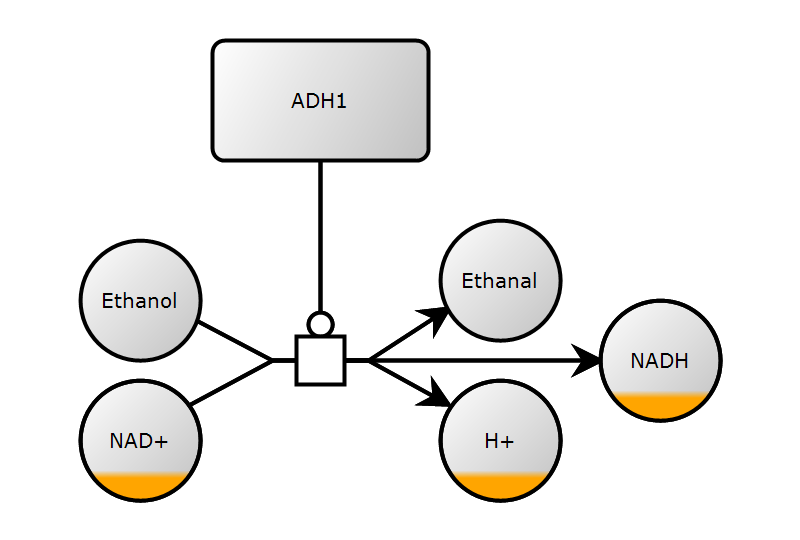
\includegraphics[width=0.4\linewidth,height=\textheight,keepaspectratio]{./images/ethanol_all.png}

\subsection{Want to know more}\label{want-to-know-more}


\includegraphics[width=0.7\linewidth,height=\textheight,keepaspectratio]{images/libsbgnpy_large.png}

\href{https://matthiaskoenig.github.io/libsbgnpy/}{libsbgnpy
documentation}




\end{document}
